\documentclass[tikz, border=15pt]{standalone}
\usepackage{amsmath, amssymb}
\usetikzlibrary{shapes.geometric, arrows.meta, positioning, fit, backgrounds, decorations.pathreplacing, calc}

\begin{document}
	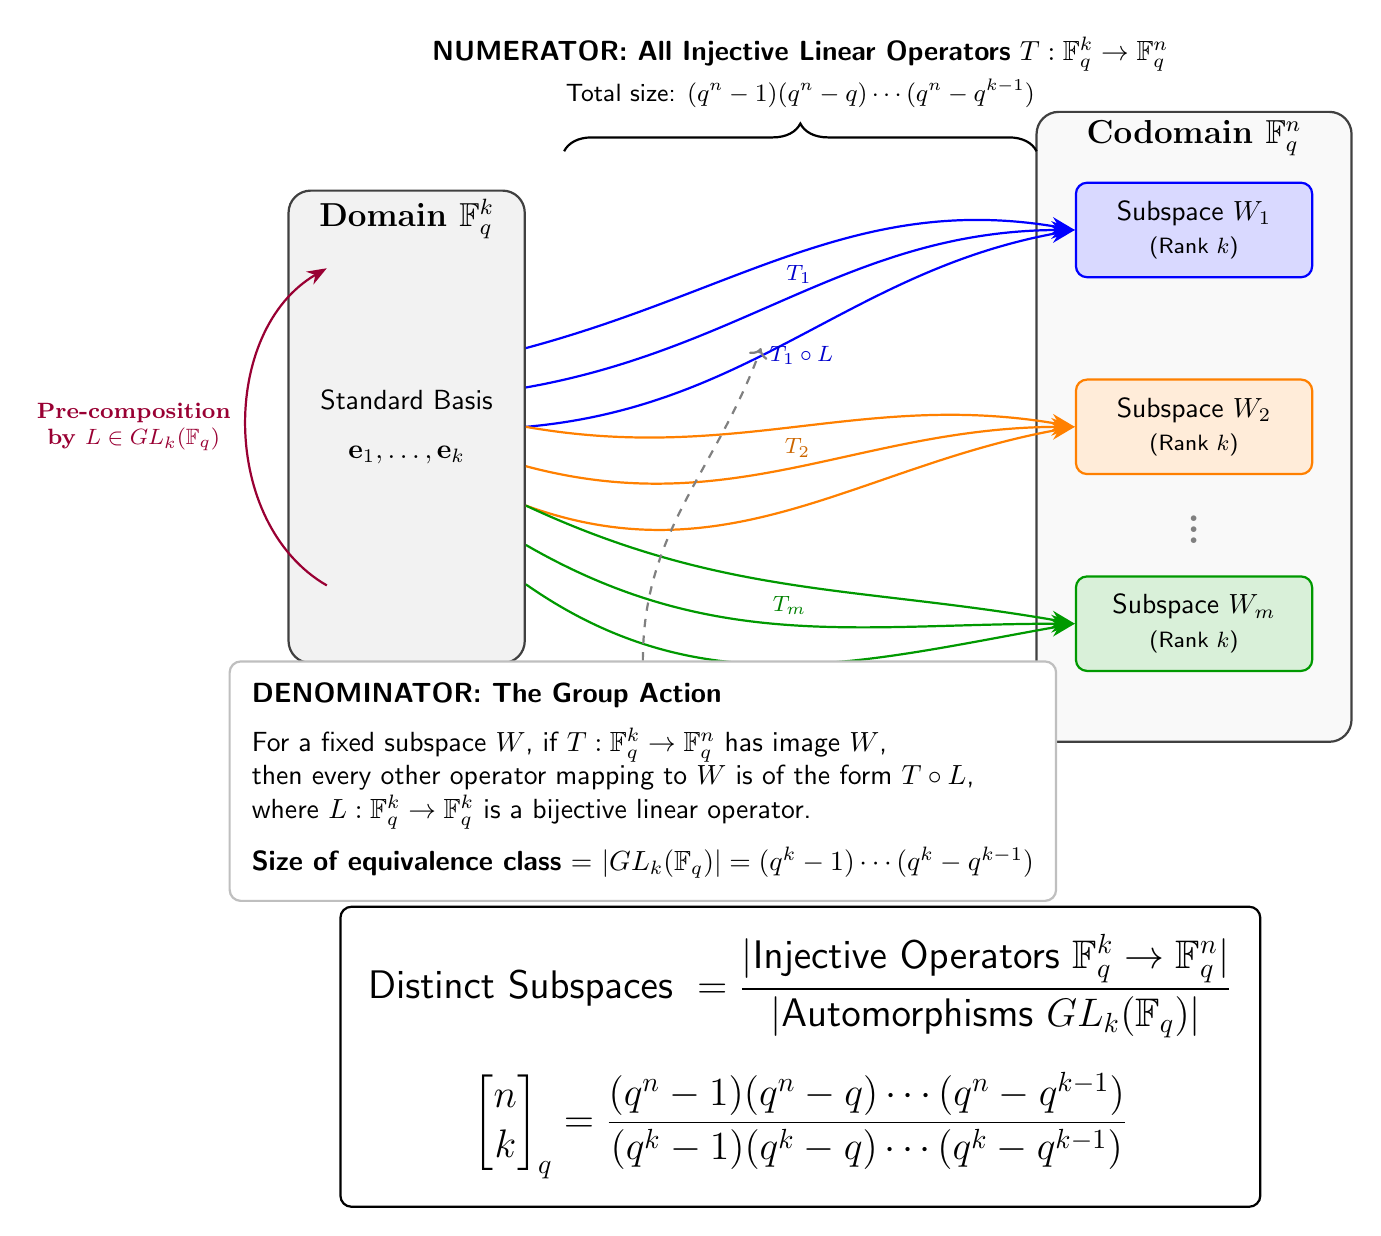
\begin{tikzpicture}[
		font=\sffamily,
		% Styles
		domainBox/.style={draw=darkgray, fill=gray!10, thick, rounded corners=8pt, minimum width=3cm, minimum height=6cm, align=center},
		codomainBox/.style={draw=darkgray, fill=gray!5, thick, rounded corners=8pt, minimum width=4cm, minimum height=8cm, align=center},
		subspaceBox/.style={draw=#1, fill=#1!15, thick, rounded corners=4pt, minimum width=3cm, minimum height=1.2cm, align=center},
		operatorArrow/.style={-{Stealth[length=3mm]}, thick, draw=#1},
		automorphismArrow/.style={-{Stealth[length=2.5mm]}, thick, draw=purple!80!black, bend left=60},
		textPanel/.style={draw=gray!50, fill=white, thick, rounded corners=4pt, inner sep=8pt, align=left}
		]
		
		% =========================================================
		% 1. SPACES (Domain and Codomain)
		% =========================================================
		% Domain F_q^k
		\node[domainBox] (Domain) at (0, 0) {};
		\node[anchor=north, font=\large\bfseries] at (Domain.north) {Domain $\mathbb{F}_q^k$};
		\node[anchor=center, align=center] at (Domain.center) {Standard Basis\\[2mm] $\mathbf{e}_1, \dots, \mathbf{e}_k$};
		
		% Codomain F_q^n
		\node[codomainBox] (Codomain) at (10, 0) {};
		\node[anchor=north, font=\large\bfseries] at (Codomain.north) {Codomain $\mathbb{F}_q^n$};
		
		% =========================================================
		% 2. DISTINCT SUBSPACES IN CODOMAIN (The "Buckets")
		% =========================================================
		\node[subspaceBox=blue] (W1) at (10, 2.5) {Subspace $W_1$\\ \footnotesize (Rank $k$)};
		\node[subspaceBox=orange] (W2) at (10, 0) {Subspace $W_2$\\ \footnotesize (Rank $k$)};
		\node[subspaceBox=green!60!black] (W3) at (10, -2.5) {Subspace $W_m$\\ \footnotesize (Rank $k$)};
		
		\node[font=\Huge, text=gray] at (10, -1.2) {\vdots};
		
		% =========================================================
		% 3. INJECTIVE OPERATORS (The Arrows / Numerator)
		% =========================================================
		% Bundle mapping to W1
		\draw[operatorArrow=blue] ($(Domain.east)+(0, 1)$) to[out=15, in=170] (W1.west);
		\draw[operatorArrow=blue] ($(Domain.east)+(0, 0.5)$) to[out=10, in=180] node[midway, above, text=blue!80!black, font=\footnotesize] {$T_1$} (W1.west);
		\draw[operatorArrow=blue] ($(Domain.east)+(0, 0)$) to[out=5, in=190] node[midway, below, text=blue!80!black, font=\footnotesize] {$T_1 \circ L$} (W1.west);
		
		% Bundle mapping to W2
		\draw[operatorArrow=orange] ($(Domain.east)+(0, 0)$) to[out=-10, in=170] (W2.west);
		\draw[operatorArrow=orange] ($(Domain.east)+(0, -0.5)$) to[out=-15, in=180] node[midway, above, text=orange!80!black, font=\footnotesize] {$T_2$} (W2.west);
		\draw[operatorArrow=orange] ($(Domain.east)+(0, -1)$) to[out=-20, in=190] (W2.west);
		
		% Bundle mapping to Wm
		\draw[operatorArrow=green!60!black] ($(Domain.east)+(0, -1)$) to[out=-25, in=170] (W3.west);
		\draw[operatorArrow=green!60!black] ($(Domain.east)+(0, -1.5)$) to[out=-30, in=180] node[midway, above, text=green!50!black, font=\footnotesize] {$T_m$} (W3.west);
		\draw[operatorArrow=green!60!black] ($(Domain.east)+(0, -2)$) to[out=-35, in=190] (W3.west);
		
		% Brace for all operators
		\draw[decorate, decoration={brace, amplitude=10pt}, thick] (2, 3.5) -- (8, 3.5) 
		node[midway, above=12pt, align=center] {
			\textbf{NUMERATOR: All Injective Linear Operators} $T: \mathbb{F}_q^k \to \mathbb{F}_q^n$\\[1mm]
			\small Total size: $(q^n-1)(q^n-q)\cdots(q^n-q^{k-1})$
		};
		
		% =========================================================
		% 4. AUTOMORPHISM GROUP ACTION (Denominator)
		% =========================================================
		% Drawing the "L" action loop on the Domain
		\draw[automorphismArrow] ($(Domain.south west)+(0.5, 1)$) to node[midway, left=2pt, align=center, text=purple!80!black, font=\footnotesize\bfseries] {Pre-composition\\by $L \in GL_k(\mathbb{F}_q)$} ($(Domain.north west)+(0.5, -1)$);
		
		\node[textPanel] (DenomPanel) at (3, -4.5) {
			\textbf{DENOMINATOR: The Group Action}\\[2mm]
			For a fixed subspace $W$, if $T: \mathbb{F}_q^k \to \mathbb{F}_q^n$ has image $W$,\\
			then every other operator mapping to $W$ is of the form $T \circ L$,\\
			where $L: \mathbb{F}_q^k \to \mathbb{F}_q^k$ is a bijective linear operator.\\[2mm]
			\textbf{Size of equivalence class} = $|GL_k(\mathbb{F}_q)| = (q^k-1)\cdots(q^k-q^{k-1})$
		};
		
		% Draw arrow from DenomPanel to the Blue bundle to indicate it represents one class
		\draw[->, thick, dashed, draw=gray] (DenomPanel.north) to[out=90, in=250] (4.5, 1);
		
		% =========================================================
		% 5. FINAL QUOTIENT EQUATION
		% =========================================================
		\node[draw=black, thick, fill=white, rounded corners=4pt, inner sep=10pt, align=center] (Formula) at (5, -8) {
			\Large $\displaystyle \text{Distinct Subspaces } = \frac{|\text{Injective Operators } \mathbb{F}_q^k \to \mathbb{F}_q^n|}{|\text{Automorphisms } GL_k(\mathbb{F}_q)|}$ \\[4mm]
			\Large $\displaystyle \begin{bmatrix} n \\ k \end{bmatrix}_q = \frac{(q^n-1)(q^n-q)\cdots(q^n-q^{k-1})}{(q^k-1)(q^k-q)\cdots(q^k-q^{k-1})}$
		};
		
	\end{tikzpicture}
\end{document}